% Roadmap-Kaskade fuer Kap. 5.3 (Vorbild: Salma Abb. 8, Grau-Optik der
% Thesis). Export:
%   pdflatex -output-directory=/tmp docs/architecture/roadmap_outlook.tex
%   cp /tmp/roadmap_outlook.pdf thesis/images/
\documentclass[border=2pt]{standalone}
\usepackage[T1]{fontenc}
\usepackage{helvet}
\renewcommand{\familydefault}{\sfdefault}
\usepackage{tikz}
\usetikzlibrary{positioning, arrows.meta}

\begin{document}
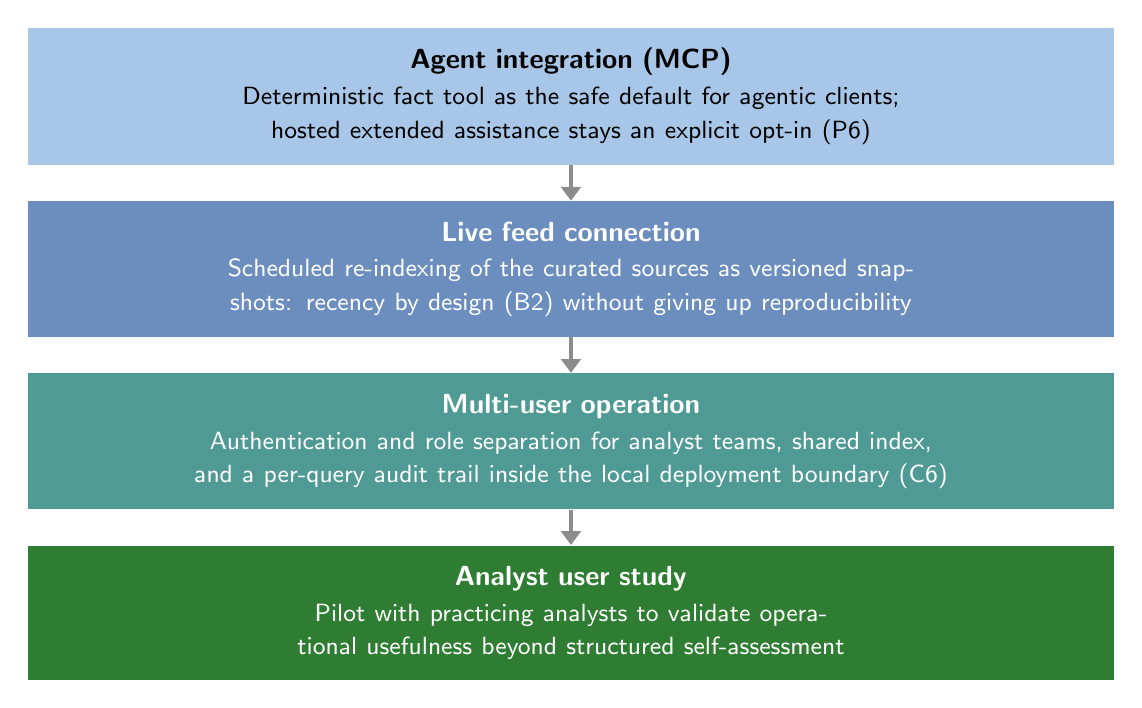
\begin{tikzpicture}[
    stage/.style={rectangle, text width=12.6cm, align=center,
                  inner xsep=6mm, inner ysep=2.6mm},
    arrow/.style={line width=1.6pt, black!45,
                  -{Triangle[length=5pt, width=7pt]}}
]
% Farbverlauf Blau -> Teal -> Gruen: gleiche Semantik wie die
% Methodik-Grafik (blaue Prozesskette, gruener Zielschritt).
\definecolor{stageblue}{HTML}{A8C7E8}
\definecolor{stagemidblue}{HTML}{6C8EBF}
\definecolor{stageteal}{HTML}{4F9A94}
\definecolor{stagegreen}{HTML}{2E7D32}
\node[stage, fill=stageblue] (s1) {%
    \textbf{Agent integration (MCP)}\\[1pt]
    {\small Deterministic fact tool as the safe default for agentic
     clients; hosted extended assistance stays an explicit opt-in
     (P6)}};
\node[stage, fill=stagemidblue, text=white, below=4.5mm of s1] (s2) {%
    \textbf{Live feed connection}\\[1pt]
    {\small Scheduled re-indexing of the curated sources as versioned
     snapshots: recency by design (B2) without giving up
     reproducibility}};
\node[stage, fill=stageteal, text=white, below=4.5mm of s2] (s3) {%
    \textbf{Multi-user operation}\\[1pt]
    {\small Authentication and role separation for analyst teams,
     shared index, and a per-query audit trail inside the local
     deployment boundary (C6)}};
\node[stage, fill=stagegreen, text=white, below=4.5mm of s3] (s4) {%
    \textbf{Analyst user study}\\[1pt]
    {\small Pilot with practicing analysts to validate operational
     usefulness beyond structured self-assessment}};

\draw[arrow] (s1.south) -- (s2.north);
\draw[arrow] (s2.south) -- (s3.north);
\draw[arrow] (s3.south) -- (s4.north);
\end{tikzpicture}
\end{document}
